\documentclass[10pt,
a4paper,
oneside,
%BCOR=25mm,
titlepage,
bibtotocnumbered,	  % Literaturverzeichnis ins Inhaltsverzeichnis
liststotocnumbered]{scrbook}
\usepackage{ngerman}
\usepackage{amsmath}
\usepackage{amsfonts}
\usepackage{amssymb}
\usepackage{graphicx}
\usepackage[colorlinks]{hyperref} 
%\usepackage[section]{glossaries} 
\usepackage[toc]{glossaries}
\makenoidxglossaries
\loadglsentries{GlossariesDef} 
\usepackage[numbers,round]{natbib}
\bibliographystyle{alphadin}
\author{Andreas Frieß}
\title{DirectShow und Lazarus}
%#### Begin des Dokumentes ####
\begin{document}
\setcounter{tocdepth}{3} %Tiefe des Inhaltsverzeichnis
%###############################################
% Umschlag und Titelseite
%###############################################
\pagestyle{empty} %%Keine Kopf-/Fusszeilen auf den ersten Seiten.
\maketitle 						% Titelei wird erzeugt
%\begin{center}
%\textbf{Andreas Frieß 2017}
%\end{center}
%\begin{quote}
%	Copyright (C) 2007-2017 Andreas Frieß.
%	Es wird die Erlaubnis gewährt, dieses Dokument zu kopieren, zu
%	verteilen und/oder zu modifizieren, unter den Bestimmungen der
%	GNU Free Documentation License, Version 1.2 oder jede spätere
%	Version, veröffentlicht von der Free Software Foundation; mit
%	keinen unveränderlichen Abschnitten, keinen vorderen
%	Umschlagtexten und keinen hinteren Umschlagtexten. Eine Kopie der
%	Lizenz ist aufgenommen in den Abschnitt mit dem Titel "GNU Free
%	Documentation License".
%	
%	Copyright \copyright{}  2007-2017 Andreas Frieß
%	Permission is granted to copy, distribute and/or modify this document
%	under the terms of the GNU Free Documentation License, Version 1.2
%	or any later version published by the Free Software Foundation;
%	with no Invariant Sections, no Front-Cover Texts, and no Back-Cover Texts.
%	A copy of the license is included in the section entitled ``GNU
%	Free Documentation License''.
%\end{quote}
%\newpage
%###############################################
% Inhaltsverzeichnis
%###############################################
%\section[Inhaltsverzeichnis]{Inhaltsverzeichnis}
\tableofcontents			% Inhaltsverzeichnis

\newpage
\pagestyle{headings} %% Kopf-/Fusszeilen aktivieren

\part[Lazarus und DirectShow]{Lazarus und DirectShow (deutsch)}
\chapter{Allgemein}
\section{Grundlagen}
\subsection{Einleitung}
\gls{DirectShow} (ehemals \"Direct Media\")\footnote{Quelle: Wikipedia\cite{400}}
DirectShow oder ehemals ActiveMovie bzw. DirectX Media dient der Verarbeitung von Video- und Audio-Dateien, womit sich verschiedenste Arten von Video-Dateien (AVI, MPEG) und Ton-Dateien (z. B. MP3) wiedergeben oder erstellen lassen. Es wird auch Streaming unterst�tzt und ist durch DirectShow-Filter beliebig erweiterbar.
DirectShow wurde inzwischen aus dem DirectX SDK entfernt und ist in das Windows Plattform-SDK aufgenommen worden. Somit geh�rt DirectShow streng genommen nicht mehr zu DirectX, sondern ist jetzt ein Bestandteil der Windows-Plattform.

Lazarus und Freepascal unterst�tzen eine vielzahl von Umgebungen, DirectShow ist eine FrameWork nur f�r Windows 32 und 64. Somit k�nnen die folgenden Informationen nur f�r Windowsversionen gelten auf denen zumindest DirectX9 oder neuer installiert ist. 

Die meisten modernen Ger�te haben bereits eine Kamera eingebaut. Diese ist intern meistens als USB-Device angeschlossen. Wie sie genau angeschlossen ist, ist f�r den Programmiere nicht relevant, solange die Kamera vom System erkannt wird und die entsprechenden Treiber von Windows geladen werden. Entweder sind die Treiber bereits generisch in Windows enthalten oder werden vom Hersteller zur Verf�gung gestellt.   

In den Beispielen wird es spezielle um Informationen gehen die sich in erster Linie mit Kameras und den verbunden Einstellungen besch�ftigt.

\subsection{Abfragen der Kategorien}
Die verschiedenen Filter sind in Kategorien eingeteilt, diese Ergeben sich aus dem Zweck der Filter und sind vom System her vorgegeben. Kategorien werden am einfachsten �ber \textbf{TSysDevEnum} aus dem Paket \textbf{DXSUtils} abgefragt. Wir lassen uns hier den lesbaren Namen \gls{FriendlyName} statt der \gls{GUID} anzeigen. Sp�ter k�nnen wir die weiteren Informationen die wir �ber \textbf{TSysDevEnum} abfragen, durch die Angabe einer \gls{GUID} auf die ben�tigten einschr�nken. 

\begin{verbatim}
unit BasicEnumCatMain;

{$mode objfpc}{$H+}

interface

uses
  Classes, SysUtils, FileUtil, Forms, Controls, Graphics, Dialogs, StdCtrls;

type

 {TBasicEnumCatForm }

TBasicEnumCatForm = class(TForm)
  BuEnum: TButton;
  LbCategories: TListBox;
  procedure BuEnumClick(Sender: TObject);
end;

var
  BasicEnumCatForm: TBasicEnumCatForm;

implementation

uses
  DXSUtil, DirectShow9;

{$R *.lfm}

  {TBasicEnumCatForm }

procedure TBasicEnumCatForm.BuEnumClick(Sender: TObject);
var
  i: integer;
  SysDev: TSysDevEnum;
begin
  SysDev:= TSysDevEnum.Create;
  try
    if SysDev.CountCategories > 0 then
      for i := 0 to SysDev.CountCategories - 1 do begin
        LbCategories.Items.Add(SysDev.Categories[i].FriendlyName);
      end;
  finally
    FreeAndNil(SysDev);
  end;
end;
end.
\end{verbatim}
Das Ergebinis siehtfolgendermassen aus:


\section{Filter}

\subsection{FilterGraph}
Der FilterGraph ist ein COM Objekt das die verschiedene Filter kontrolliert und viele zus�tzlichen Funktionen durchf�hrt. Das sind zum Beispiel 
\begin{itemize}
	\item Koordinieren von Status �ber die Filtergrenzen hinweg
	\item Bereitstellen eines Referenztaktgebers 
	\item Kommunikation mit dem Programm �ber Callbacks
	\item Methoden und Funktionen zum erstellen des Filtergraphs
\end{itemize}


\subsection{WebCam}



Das ist ein Platzhalter

\gls{Moniker}


\part[DirectShow]{DirectShow (english)}
%###########################################################
% Einführung, Therorie, ....
%###########################################################
%--------------------------------------------------
% Alles was allgemeine Information ist
%--------------------------------------------------
\chapter{Microsoft Articles}
\section{DirectShow System Overview }\footnote{Quelle: \cite{500}}
%####################################################################
%    Copyright @ 2007-2017 Andreas Frie� (Friess)
%    Permission is granted to copy, distribute and/or modify this document
%    under the terms of the GNU Free Documentation License, Version 1.2
%    or any later version published by the Free Software Foundation;
%    with no Invariant Sections, no Front-Cover Texts, and no Back-Cover Texts.
%    A copy of the license is included in the section entitled ``GNU
%    Free Documentation License''.
%%####################################################################
% Created: 24.05.2017
%%####################################################################
% !!!!! Copyrighted Text !!!!!! from
% https://msdn.microsoft.com/de-de/library/windows/desktop/dd375470(v=vs.85).aspx
%%####################################################################

\subsection{The Challenge of Multimedia}
Working with multimedia presents several major challenges:
\begin{itemize}
	\item Multimedia streams contain large amounts of data, which must be processed very quickly.
\item Audio and video must be synchronized so that it starts and stops at the same time, and plays at the same rate.
\item Data can come from many sources, including local files, computer networks, television broadcasts, and video cameras.
\item Data comes in a variety of formats, such as Audio-Video Interleaved (AVI), Advanced Streaming Format (ASF), Motion Picture Experts Group (MPEG), and Digital Video (DV).
\item The programmer does not know in advance what hardware devices will be present on the end-user's system.
\end{itemize}
\subsection{The DirectShow Solution}
DirectShow is designed to address each of these challenges. Its main design goal is to simplify the task of creating digital media applications on the Windows platform, by isolating applications from the complexities of data transports, hardware differences, and synchronization.
\\To achieve the throughput needed to stream video and audio, DirectShow uses Direct3D and DirectSound whenever possible. These technologies render data efficiently to the user's sound and graphics cards. DirectShow synchronizes playback by encapsulating media data in time-stamped samples. To handle the variety of sources, formats, and hardware devices that are possible, DirectShow uses a modular architecture, in which the application mixes and matches different software components called filters.
\\DirectShow provides filters that support capture and tuning devices based on the Windows Driver Model (WDM), as well as filters that support older Video for Windows (VfW) capture cards, and codecs written for the Audio Compression Manager (ACM) and Video Compression Manager (VCM) interfaces.
\\The following diagram \ref{fig:ic420381} shows the relationship between an application, the DirectShow components, and some of the hardware and software components that DirectShow supports.
\begin{figure}[!ht]
	\centering
	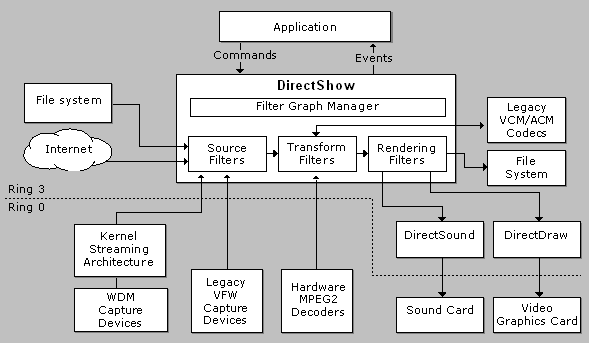
\includegraphics[width=0.7\linewidth]{ms_pic/IC420381}
	\caption{Relationship between application and DirectShow }
	\label{fig:ic420381}
\end{figure}
As illustrated here, DirectShow filters communicate with, and control, a wide variety of devices, including the local file system, TV tuner and video capture cards, VfW codecs, the video display (through DirectDraw or GDI), and the sound card (through DirectSound). Thus, DirectShow insulates the application from many of the complexities of these devices. DirectShow also provides native compression and decompression filters for certain file formats.


\section{The Filter Graph and Its Components}\footnote{Quelle: \cite{501}}
%####################################################################
%    Copyright @ 2007-2017 Andreas Frie� (Friess)
%    Permission is granted to copy, distribute and/or modify this document
%    under the terms of the GNU Free Documentation License, Version 1.2
%    or any later version published by the Free Software Foundation;
%    with no Invariant Sections, no Front-Cover Texts, and no Back-Cover Texts.
%    A copy of the license is included in the section entitled ``GNU
%    Free Documentation License''.
%%####################################################################
% Created: 24.05.2017
%%####################################################################
% !!!!! Copyrighted Text !!!!!! from
% https://msdn.microsoft.com/de-de/library/windows/desktop/dd375470(v=vs.85).aspx
%%####################################################################
This article describes the major components of DirectShow. It is intended as an introduction for application developers and for developers writing custom DirectShow filters. Application developers can usually ignore many of the low-level details of DirectShow. However, it is still a good idea to read this section, to have a general understanding of the DirectShow architecture.

\subsection{About DirectShow Filters}
DirectShow uses a modular architecture, where each stage of processing is done by a COM object called a filter. DirectShow provides a set of standard filters for applications to use, and developers can write their own custom filters that extend the functionality of DirectShow. To illustrate, here are the steps needed to play an AVI video file, along with the filters that perform each step:
\begin{itemize}
	\item Read the raw data from the file as a byte stream (File Source filter).
	\item Examine the AVI headers, and parse the byte stream into separate video frames and audio samples (AVI Splitter filter).
	\item Decode the video frames (various decoder filters, depending on the compression format).
	\item Draw the video frames (Video Renderer filter).
	\item Send the audio samples to the sound card (Default DirectSound Device filter).
\end{itemize}
These filters are shown in the following diagram \ref{fig:ic420231}.
\begin{figure}[!h]
	\centering
	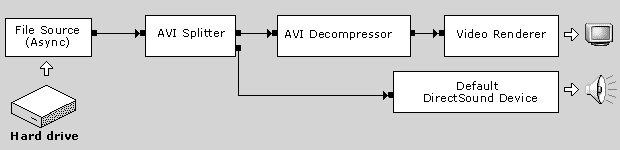
\includegraphics[width=0.7\linewidth]{ms_pic/IC420231}
	\caption{Filter Graph for playback}
	\label{fig:ic420231}
\end{figure}
Filter graph for playing back an AVI file with compressed video
As the diagram shows, each filter is connected to one or more other filters. The connection points are also COM objects, called \textit{pins}. Filters use pins to move data from one filter the next. The arrows in the diagram show the direction in which the data travels. In DirectShow, a set of filters is called a \textit{filter graph}.
\\Filters have three possible states: running, stopped, and paused. When a filter is running, it processes media data. When it is stopped, it stops processing data. The paused state is used to cue data before running; the section Data Flow in the Filter Graph describes this concept in more detail. With very rare exceptions, state changes are coordinated throughout the entire filter graph; all the filters in the graph switch states in unison. Thus, the entire filter graph is also said to be running, stopped, or paused.
Filters can be grouped into several broad categories:
\begin{itemize}
	\item A source filter introduces data into the graph. The data might come from a file, a network, a camera, or anywhere else. Each source filter handles a different type of data source.
	\item A transform filter takes an input stream, processes the data, and creates an output stream. Encoders and decoders are examples of transform filters.
	\item Renderer filters sit at the end of the chain. They receive data and present it to the user. For example, a video renderer draws video frames on the display; an audio renderer sends audio data to the sound card; and a file-writer filter writes data to a file.
	\item A splitter filter splits an input stream into two or more outputs, typically parsing the input stream along the way. For example, the AVI Splitter parses a byte stream into separate video and audio streams.
	\item A mux filter takes multiple inputs and combines them into a single stream. For example, the AVI Mux performs the inverse operation of the AVI Splitter. It takes audio and video streams and produces an AVI-formatted byte stream.
\end{itemize}
The distinctions between these categories are not absolute. For example, the ASF Reader filter acts as both a source filter and a splitter filter.
//All DirectShow filters expose the IBaseFilter interface, and all pins expose the IPin interface. DirectShow also defines many other interfaces that support more specific functionality.

\subsection{About the Filter Graph Manager}\footnote{Quelle: \cite{502}}
The Filter Graph Manager is a COM object that controls the filters in a filter graph. It performs many functions, including the following:
\begin{itemize}
	\item Coordinating state changes among the filters.
	\item Establishing a reference clock.
	\item Communicating events back to the application.
	\item Providing methods for applications to build the filter graph.
\end{itemize}
Each of these functions is described briefly here. Details can be found elsewhere in the documentation.


\begin{description}
	\item[State changes] State changes within filters must occur in a particular order. Therefore, the application does not issue state-change commands directly to the filters. Instead, it gives a single command to the Filter Graph Manager, which distributes the command to each of the filters. Seeking works in a similar fashion: The application gives a seek command to the Filter Graph Manager, which distributes it to the filters.
  	\item[Reference clock] All of the filters in the graph use the same clock, called a reference clock. The reference clock ensures that all the streams are synchronized. The time at which a video frame or audio sample should be rendered is called the presentation time. The presentation time is measured relative to the reference clock. The Filter Graph Manager chooses a reference clock, usually either the clock on the sound card, or the system clock.
	\item[Graph events] The Filter Graph Manager uses an event queue to inform the application of events that occur in the filter graph. This mechanism is similar to a Windows message loop.
	\item[Graph-building methods] The Filter Graph Manager provides methods for the application to add filters to the graph, connect filters to other filters, and disconnect filters.
\end{description}One function the Filter Graph Manager does not handle is moving data from one filter to the next. This is done by the filters themselves, through their pin connections. Processing always happens on a separate thread.
\begin{verse}
	\textbf{Note}\emph{  Filters are always free-threaded, reside in the same process as the Filter Graph Manager, and are loaded from in-process servers. Therefore, method calls are not marshaled between filters, or between filters and the Filter Graph Manager.}
\end{verse}

\subsection{About Media Types}
Because DirectShow is modular, it requires a way to describe the format of the data at each point in the filter graph. For example, consider AVI playback. Data enters the graph as a stream of RIFF chunks. These are parsed into video and audio streams. The video stream consists of video frames, which are probably compressed. After decoding, the video stream is a series of uncompressed bitmaps. The audio stream goes through a similar process.\\
Media Types: How DirectShow Represents Formats\\
The media type is a universal and extensible way to describe digital media formats. When two filters connect, they agree on a media type. The media type identifies what kind of data the upstream filter will deliver to the downstream filter, and the physical layout of the data. If two filters cannot agree on a media type, they will not connect.\\
For some applications, you will never have to worry about media types. In file playback, for example, DirectShow handles all of the details. Other kinds of applications may need to work directly with media types.\\
Media types are defined using the AM\_MEDIA\_TYPE structure. This structure contains the following information:
\begin{description}
	\item[Major type] The major type is a GUID that defines the overall category of the data. Major types include video, audio, unparsed byte stream, MIDI data, and so forth.
	\item[Subtype] The subtype is another GUID, which further defines the format. For example, within the video major type, there are subtypes for RGB-24, RGB-32, UYVY, and so forth. Within audio, there is PCM audio, MPEG-1 payload, and others. The subtype provides more information than the major type, but it does not define everything about the format. For example, video subtypes do not define the image size or the frame rate. These are defined by the format block, described below.
	\item[Format block] The format block is a block of data that describes the format in detail. The format block is allocated separately from the AM\_MEDIA\_TYPE structure. The pbFormat member of the AM\_MEDIA\_TYPE structure points to the format block.
\end{description}The pbFormat member is typed void* because the layout of the format block changes depending on the media type. For example, PCM audio uses a WAVEFORMATEX structure. Video uses various structures, including VIDEOINFOHEADER and VIDEOINFOHEADER2. The formattype member of the AM\_MEDIA\_TYPE structure is a GUID that specifies which structure is contained in the format block. Each format structure is assigned a GUID. The cbFormat member specifies the size of the format block. Always check these values before dereferencing the pbFormat pointer.\\
If the format block is filled in, then the major type and subtype contain redundant information. The major type and subtype, however, provide a convenient way to identify formats without a complete format block. For example, you can specify a generic 24-bit RGB format (MEDIASUBTYPE\_RGB24), without knowing all of the information required by the VIDEOINFOHEADER structure, such as image size and frame rate.\\
For example, a filter might use the following code to check a media type:

\begin{verbatim}
C++

HRESULT CheckMediaType(AM_MEDIA_TYPE *pmt)
{
    if (pmt == NULL) return E_POINTER;

    // Check the major type. We're looking for video.
    if (pmt->majortype != MEDIATYPE_Video)
    {
        return VFW_E_INVALIDMEDIATYPE;
    }

    // Check the subtype. We're looking for 24-bit RGB.
    if (pmt->subtype != MEDIASUBTYPE_RGB24)
    {
        return VFW_E_INVALIDMEDIATYPE;
    }

    // Check the format type and the size of the format block.
    if ((pmt->formattype == FORMAT_VideoInfo) &&
        (pmt->cbFormat >= sizeof(VIDEOINFOHEADER) &&
        (pmt->pbFormat != NULL))
    {
        // Now it's safe to coerce the format block pointer to the
        // correct structure, as defined by the formattype GUID.
        VIDEOINFOHEADER *pVIH = (VIDEOINFOHEADER*)pmt->pbFormat;

        // Examine pVIH (not shown). If it looks OK, return S_OK.
        return S_OK;
    }

    return VFW_E_INVALIDMEDIATYPE;
}
\end{verbatim}
The AM\_MEDIA\_TYPE structure also contains some optional fields. These can be used to provide additional information, but filters are not required to use them:
\begin{description}
	\item[lSampleSize] If this field is non-zero, it defines the size of each sample. If it is zero, it indicates that the sample size may change from sample to sample.
	\item[bFixedSizeSamples] If this Boolean flag is TRUE, it means the value in \textbf{lSampleSize} is valid. Otherwise, you should ignore \textbf{lSampleSize}.
	\item[bTemporalCompression] If this Boolean flag is FALSE, it means that all frames are key frames.
\end{description}

\subsection{About Media Samples and Allocators}
Filters deliver data across pin connections. Data moves from the output pin of one filter to the input pin of another filter. The most common way for the output pin to deliver the data is by calling the IMemInputPin::Receive method on the input, although a few other mechanisms exist as well.\\
Depending on the filter, memory for the media data can be allocated in various ways: on the heap, in a DirectDraw surface, using shared GDI memory, or using some other allocation mechanism. The object responsible for allocating the memory is called an allocator, which is a COM object that exposes the IMemAllocator interface.\\
When two pins connect, one of the pins must provide an allocator. DirectShow defines a sequence of method calls that is used to establish which pin provides the allocator. The pins also agree on the number of buffers that the allocator will create, and the size of the buffers.\\
Before streaming begins, the allocator creates a pool of buffers. During streaming, the upstream filter fills buffers with data and delivers them to the downstream filter. But the upstream filter does not give the downstream filter raw pointers to the buffers. Instead, it uses COM objects called media samples, which the allocator creates to manage the buffers. Media samples expose the IMediaSample interface. A media sample contains:
\begin{enumerate}
	\item a pointer to the underlying buffer
	\item a time stamp
	\item various flags
	\item optionally, a media type
\end{enumerate}
The time stamp defines the presentation time, which the renderer filter uses to schedule rendering. The flags indicate things like whether there was a break in the data since the previous sample. The media type provides a way for filters to change formats mid-stream. Usually, the sample has no media type, which indicates that the format has not changed since the previous sample.\\
While a filter is using a buffer, it holds reference count on the sample. The allocator uses the reference count to determine when it can re-use the buffer. This prevents a filter from overwriting a buffer that another filter is still using. A sample does not return to the allocator's pool of available samples until every filter has released it.\\
For more information, see the following topics:
\begin{itemize}
	\item The topic Samples and Allocators provides a more detailed description of how allocators work.
	\item The topic Data Flow in the Filter Graph gives a general overview of data flow in DirectShow.
\end{itemize}
The following topics are intended for developers who are writing their own custom filters:
\begin{itemize}
	\item Data Flow for Filter Developers
	\item Threads and Critical Sections
\end{itemize}

\subsection{How Hardware Devices Participate in the Filter Graph}
This article describes how DirectShow interacts with audio and video hardware.
\paragraph{Wrapper Filters}
All DirectShow filters are user mode software components. In order for a kernel mode hardware device, such as a video capture card, to join a DirectShow filter graph, the device must be represented as a user-mode filter. This function is performed by specialized \"wrapper\" filters provided with DirectShow. These filters include the Audio Capture filter, the VFW Capture filter, the TV Tuner filter, the TV Audio filter, and the Analog Video Crossbar filter. DirectShow also provides a filter called KsProxy, which can represent any type of Windows Driver Model (WDM) streaming device. Hardware vendors can extend KsProxy to support custom functionality, by providing a Ksproxy plug-in, which is a COM object aggregated by KsProxy.//
The wrapper filters expose COM interfaces that represent the capabilities of the device. The application uses these interfaces to pass information to and from the filter. The filter translates the COM method calls into device driver calls, passes that information to the driver in kernel mode, and then translates the result back to the application. The TV Tuner, TV Audio, Analog Video Crossbar, and KsProxy filters support custom driver properties through the IKsPropertySet interface. The VFW Capture filter and the Audio Capture filter are not extensible in this way.//
For application developers, wrapper filters enable the application to control devices just as they control any other DirectShow filter. No special programming is required; the details of communicating with the kernel-mode device are encapsulated within the filter.
\paragraph{Video for Windows Devices}
The VFW Capture filter supports earlier Video for Windows (VfW) capture cards. When a VfW card is present on the target system, it can be discovered and added to the filter graph using the DirectShow System Device Enumerator. For details, see Enumerating Devices and Filters.
\paragraph{Audio Capture and Mixing Devices (Sound Cards)}
Newer sound cards have input jacks for microphones and other types of devices. Typically these cards also have on-board mixing capabilities for controlling the volume, treble, and bass of each individual input. In DirectShow, the sound card's inputs and mixer are wrapped by the Audio Capture filter. Each sound card can be discovered with the System Device Enumerator. To view the sound cards in your system, run GraphEdit and select from the Audio Capture Sources category. Each filter in that category is a separate instance of the Audio Capture filter. (See Using GraphEdit.)
\paragraph{WDM Streaming Devices}
Newer hardware decoders and capture cards conform to the Windows Driver Model (WDM) specification. These devices have greater functionality than VfW devices. WDM video capture cards can support features that are not available under VfW, including the enumeration of capture formats, programmatic control of video parameters such as hue and brightness, programmatic input selection, and TV Tuner support.//
To support WDM streaming devices, DirectShow provides the KsProxy filter (ksproxy.ax). KsProxy has been called the \"Swiss Army Knife filter\" because it does so many different things. The number of pins on the filter, and the number of COM interfaces exposed by the filter, depend on the capabilities of the underlying driver. KsProxy does not appear in the filter graph under the name \"KsProxy.\" It always takes the friendly name of the device, which is found in the registry. To view the WDM devices on your system, run GraphEdit and select from the WDM Streaming categories. Even if you have only one WDM card on your system, that card might contain more than one device. Each device is represented as a separate filter, and each of these filters is actually KsProxy.//
An application uses the System Device Enumerator to find WDM device monikers on the system. KsProxy is instantiated by calling \textbf{BindToObject} on the moniker. Because KsProxy can represent all kinds of WDM devices, it must query the driver to determine which property sets the driver supports. Property sets are collections of data structures used by WDM drivers, and also by some user mode filters, such as MPEG-2 software decoders. KsProxy configures itself to expose the COM interfaces that correspond to those property sets. KsProxy translates the COM method calls into property sets and sends these to the driver. Hardware vendors can extend KsProxy by supplying plug-ins, which are vendor-specific interfaces that expose the special capabilities of a device. All these details are hidden from application. The application controls the device by way of KsProxy, in the same way as any other DirectShow filter.
\paragraph{Kernel Streaming}
WDM devices support kernel streaming, in which data is streamed entirely in kernel mode without ever switching to user mode. Switching between kernel mode and user mode is computationally expensive; kernel streaming allows for high bit rates without burdening the host CPU. WDM-based filters can use kernel streaming to pass multimedia data directly from one hardware device to another, either on the same card or on a different card, without copying the data into the system's main memory.//
From an application's point of view, it appears as if the data moves from one user-mode filter to the next. In reality, the data might never pass into user mode at all, but instead might be streamed directly from one kernel-mode device to another until it is rendered on the video graphics card. Some scenarios, such as capture to a file, require that the data pass from kernel mode to user mode at some point. However, this switch does not necessarily require the data to be copied to a new location in memory.//
Application developers generally do not need to be concerned with the details of kernel streaming, except as background information. See the Microsoft DDK for more detailed information about WDM, kernel streaming, KsProxy, and related topics.



\section{Basic DirectShow Tasks}
\subsection{Displaying a Filter's Property Pages}
\textbf{Displaying a Filter's Property Pages}

A property page is one way for a filter to support properties that the user can set. This article describes how to display a filter's property pages in an application. For more information about property pages, see the Platform SDK documentation.

\begin{description}
	\item[Note]  Although many of the filters provided with DirectShow support property pages, they are intended for debugging purposes, and are not recommended for application use. In most cases the equivalent functionality is provided through a custom interface on the filter. An application should control these filters programmatically, rather than expose their property pages to users.
\end{description}

Filters with property pages expose the ISpecifyPropertyPages interface. To determine whether a filter defines a property page, query the filter for this interface using QueryInterface.
If you directly created an instance of a filter (by calling CoCreateInstance), you already have a pointer to the filter. If not, you can enumerate the filters in the graph, using the IFilterGraph::EnumFilters method. For details, see Enumerating Objects in a Filter Graph.

Once you have the ISpecifyPropertyPages interface pointer, retrieve the filter's property pages by calling the ISpecifyPropertyPages::GetPages method. This method fills a counted array of globally unique identifiers (GUIDs) with the class identifier (CLSID) of each property page. A counted array is defined by a CAUUID structure, which you must allocate but do not have to initialize. The GetPages method allocates the array, which is contained in the pElems member of the CAUUID structure. When you are done, free the array by calling the CoTaskMemFree function.

The OleCreatePropertyFrame function provides a simple way to display the property pages inside a modal dialog box.

\begin{verbatim}
C++

IBaseFilter *pFilter;
/* Obtain the filter's IBaseFilter interface. (Not shown) */
ISpecifyPropertyPages *pProp;
HRESULT hr = pFilter->QueryInterface(IID_ISpecifyPropertyPages, (void **)&pProp);
if (SUCCEEDED(hr)) 
{
	// Get the filter's name and IUnknown pointer.
	FILTER_INFO FilterInfo;
	hr = pFilter->QueryFilterInfo(&FilterInfo); 
	IUnknown *pFilterUnk;
	pFilter->QueryInterface(IID_IUnknown, (void **)&pFilterUnk);
	
	// Show the page. 
	CAUUID caGUID;
	pProp->GetPages(&caGUID);
	pProp->Release();
	OleCreatePropertyFrame(
	hWnd,                   // Parent window
	0, 0,                   // Reserved
	FilterInfo.achName,     // Caption for the dialog box
	1,                      // Number of objects (just the filter)
	&pFilterUnk,            // Array of object pointers. 
	caGUID.cElems,          // Number of property pages
	caGUID.pElems,          // Array of property page CLSIDs
	0,                      // Locale identifier
	0, NULL                 // Reserved
	);
	
	// Clean up.
	pFilterUnk->Release();
	FilterInfo.pGraph->Release(); 
	CoTaskMemFree(caGUID.pElems);
}

\end{verbatim}
\section{DirectShow Reference}
\subsection{Constants and GUIDs}


\subsubsection{Merit}
\gls{merit} values define the order in which the Filter Graph Manager tries to add filters during graph building.

\begin{description}
	\item[label] description
	\item [MERIT\_PREFERRED] (0x800000)
	\item [MERIT\_NORMAL] (0x600000)
	\item [MERIT\_UNLIKELY] (0x400000)
	\item [MERIT\_DO\_NOT\_USE] (0x200000)
	\item [MERIT\_SW\_COMPRESSOR] (0x100000)
	\item [MERIT\_HW\_COMPRESSOR] (0x100050)
\end{description}

\paragraph{Remarks}
Each filter is registered with a merit value. When the filter graph manager builds a graph, it enumerates all the filters registered with the correct media type. Then it tries them in order of merit, from highest to lowest. (It uses additional criteria to choose between filters with equal merit.) It never tries filters with a merit value less than or equal to \textbf{MERIT\_DO\_NOT\_USE}.
A filter that should never be considered for ordinary playback should have a merit of \textbf{MERIT\_DO\_NOT\_USE} or less. Filters can be registered with intermediate values not defined by this enumeration, such as \textbf{MERIT\_NORMAL} + 1.

\paragraph{Requirements}

\begin{tabular}[h]{|l|l|}
	\hline
	\textbf{Header} & Dshow.h\\
	\hline
\end{tabular}

	

\section{Video Capture Tasks}
\subsection{Configure the Video Quality}
This topic describes how an application can programmatically change the image and camera settings on a video capture device.

\begin{itemize}
	\item ProcAmp Settings
	\item Camera Settings
	\item Related topics
	\item ProcAmp Settings
\end{itemize}

Windows Driver Model (WDM) video cameras can support properties that control the quality of the image:

\begin{itemize}
	\item 	\item Backlight compensation
	\item Brightness
	\item Contrast
	\item Gain
	\item Gamma
	\item Hue
	\item Saturation
	\item Sharpness
	\item White balance

\end{itemize}
These properties are controlled through the IAMVideoProcAmp interface. Use this interface as follows:
Call QueryInterface on the capture filter for the IAMVideoProcAmp interface.

For each property that you want to set, call the IAMVideoProcAmp::GetRange method. Properties are specified by the VideoProcAmpProperty enumeration. If the GetRange method fails, it means the camera does not support that particular property.

If GetRange succeeds, it returns the range of supported values for the property, the default value, and the minimum increment.

To get the current value of a property, call IAMVideoProcAmp::Get.

To set a property, call the IAMVideoProcAmp::Set method. To restore a property to its default value, call GetRange to find the default and pass that value to the Set method.

You do not have to stop the filter graph when you set the properties.

The following code configures a trackbar control so that it can be used to set the brightness. The range of the trackbar corresponds to the brightness range that the device supports, and position of the trackbar corresponds to the device's initial brightness setting.

\begin{verbatim}
C++

HWND hTrackbar; // Handle to the trackbar control. 
// Initialize hTrackbar (not shown).

// Query the capture filter for the IAMVideoProcAmp interface.
IAMVideoProcAmp *pProcAmp = 0;
hr = pCap->QueryInterface(IID_IAMVideoProcAmp, (void**)&pProcAmp);
if (FAILED(hr))
{
    // The device does not support IAMVideoProcAmp, so disable the control.
    EnableWindow(hTrackbar, FALSE);
}
else
{
    long Min, Max, Step, Default, Flags, Val;
	
    // Get the range and default value. 
    hr = m_pProcAmp->GetRange(VideoProcAmp_Brightness, &Min, &Max, &Step, &Default, &Flags);
    if (SUCCEEDED(hr))
    {
        // Get the current value.
        hr = m_pProcAmp->Get(VideoProcAmp_Brightness, &Val, &Flags);
    }
    if (SUCCEEDED(hr))
    {
        // Set the trackbar range and position.
        SendMessage(hTrackbar, TBM_SETRANGE, TRUE, MAKELONG(Min, Max));
        SendMessage(hTrackbar, TBM_SETPOS, TRUE, Val);
        EnableWindow(hTrackbar, TRUE);
    }
    else
    {
        // This property is not supported, so disable the control.
        EnableWindow(hTrackbar, FALSE);
    }
}
\end{verbatim}

Camera Settings

The IAMCameraControl interface is similar to IAMVideoProcAmp, but controls various setttings on the camera itself:
\begin{itemize}
    \item Exposure
    \item Focus
    \item Iris
    \item Pan
    \item Roll
    \item Tilt
    \item Zoom
\end{itemize}
To use this interface, follow the same steps used for IAMVideoProcAmp:

Query the capture filter for the IAMCameraControl.

Call IAMCameraControl::GetRange to find which settings are supported, and the possible range for each settings.

Call IAMCameraControl::Get to get the current value of a setting.

Call IAMCameraControl::Set to set the value.

%--------------------------------------------------
% Strukturen von DirectShow
%--------------------------------------------------
\section{DirectShow Structures}
\subsection{AM\_MEDIA\_TYPE structure}\footnote{Quelle:\cite{504}}
The AM\_MEDIA\_TYPE structure describes the format of a media sample.
\paragraph{Syntax}
\begin{verbatim}
C++

typedef struct \_MediaType {
        GUID     majortype;
        GUID     subtype;
        BOOL     bFixedSizeSamples;
        BOOL     bTemporalCompression;
        ULONG    lSampleSize;
        GUID     formattype;
        IUnknown *pUnk;
        ULONG    cbFormat;
    BYTE     *pbFormat;
    } AM\_MEDIA\_TYPE;
\end{verbatim}
\paragraph{Members}

\begin{description}
	\item[majortype]
Globally unique identifier (GUID) that specifies the major type of the media sample. For a list of possible major types, see Media Types.
	\item[subtype] GUID that specifies the subtype of the media sample. For a list of possible subtypes, see Media Types. For some formats, the value might be MEDIASUBTYPE\_None, which means the format does not require a subtype.
	\item[bFixedSizeSamples] If TRUE, samples are of a fixed size. This field is informational only. For audio, it is generally set to TRUE. For video, it is usually TRUE for uncompressed video and FALSE for compressed video.
	\item[bTemporalCompression] If TRUE, samples are compressed using temporal (interframe) compression. A value of TRUE indicates that not all frames are key frames. This field is informational only.
	\item[lSampleSize] Size of the sample in bytes. For compressed data, the value can be zero.
	\item[formattype] GUID that specifies the structure used for the format block. The pbFormat member points to the corresponding format structure. Format types include the following:\\ \\
\begin{tabular}[h]{||l|l||}
		\hline \hline
	Format type & Format structure \\ \hline
	FORMAT\_DvInfo & DVINFO \\ \hline
	FORMAT\_MPEG2Video &	MPEG2VIDEOINFO \\ \hline
	FORMAT\_MPEGStreams & AM\_MPEGSYSTEMTYPE \\ \hline
	FORMAT\_MPEGVideo & MPEG1VIDEOINFO \\ \hline
	FORMAT\_None &	None \\ \hline
	FORMAT\_VideoInfo & VIDEOINFOHEADER \\ \hline
	FORMAT\_VideoInfo2 &	VIDEOINFOHEADER2 \\ \hline
	FORMAT\_WaveFormatEx & WAVEFORMATEX \\ \hline
	GUID\_NULL &	None \\
	\hline \hline
\end{tabular}
	\item[pUnk] Not used. Set to NULL.
	\item[cbFormat] Size of the format block, in bytes.
	\item[pbFormat] Pointer to the format block. The structure type is specified by the formattype member. The format structure must be present, unless \textbf{formattype} is GUID\_NULL or FORMAT\_None.\\The \textbf{pbFormat} buffer must be allocated by calling CoTaskMemAlloc. To release the format block, call \textbf{FreeMediaType}.	
\end{description}

\paragraph{Remarks}

When two pins connect, they negotiate a media type, which is defined by an AM\_MEDIA\_TYPE structure. The media type describes the format of the data that the filters will exchange. If the filters do not agree on a media type, they cannot connect.
The stream type is specified by two GUIDs, called the major type and the subtype. The major type defines the general category, such as video, audio, or byte stream. The subtype defines a narrower category within the major type. For example, video subtypes include 8-bit, 16-bit, 24-bit, and 32-bit RGB.\\
The AM\_MEDIA\_TYPE structure is followed by a variable-length block of data that contains format-specific information. The pbFormat member points to this block, called the format block. The layout of the format block depends on the type of data in the stream, and is specified by the formattype member. The format block might be NULL. Check the cbFormat member to determine the size. Cast the pbFormat member to access the format block. For example:

\begin{verbatim}
C++

if (pmt->formattype == FORMAT\_VideoInfo)
{
    // Check the buffer size.
    if (pmt->cbFormat >= sizeof(VIDEOINFOHEADER))
    {
        VIDEOINFOHEADER *pVih = 
        reinterpret\_cast<VIDEOINFOHEADER*>(pmt->pbFormat);
        /* Access VIDEOINFOHEADER members through pVih. */
    }
}
\end{verbatim}
\paragraph{Requirements}
\begin{tabular}[h]{|l|l|}
	\hline
	HeaderL & Strmif.h (include Dshow.h)\\
	\hline
\end{tabular}





\part{The Component Object Model - COM}
\chapter{COM fundamentals}
\section{Monikers}
\textbf{Monikers}

A moniker in COM is not only a way to identify an object?a moniker is also implemented as an object. This object provides services allowing a component to obtain a pointer to the object identified by the moniker. This process is referred to as binding.

Monikers are objects that implement the IMoniker interface and are generally implemented in DLLs as component objects. There are two ways of viewing the use of monikers: as a moniker client, a component that uses a moniker to get a pointer to another object; and as a moniker provider, a component that supplies monikers identifying its objects to moniker clients.

OLE uses monikers to connect to and activate objects, whether they are in the same machine or across a network. A very important use is for network connections. They are also used to identify, connect to, and run OLE compound document link objects. In this case, the link source acts as the moniker provider and the container holding the link object acts as the moniker client.

For more information, see the following topics:
\begin{list}{label}{spacing}
	\item Moniker Clients
	\item Moniker Providers
	\item OLE Moniker Implementations
\end{list}

%###########################################################
% Verzeichnisse,....
%###########################################################
% chapter Verzeichnis der Bilder
\listoffigures
% Chapter Verzeichnis der Tabellen
\listoftables
% Ausgabe Bibligraphy
\bibliography{DirectShow}
% Ausgabe des Glossares
\printnoidxglossaries
\end{document}